\setauthor{Abdulrahman Al Sabagh}
\section{\textbf{E}ntity \textbf{R}elationship \textbf{D}iagram (ERD)}
\begin{spacing}{1}

  \begin{figure}[H]
    \centering
    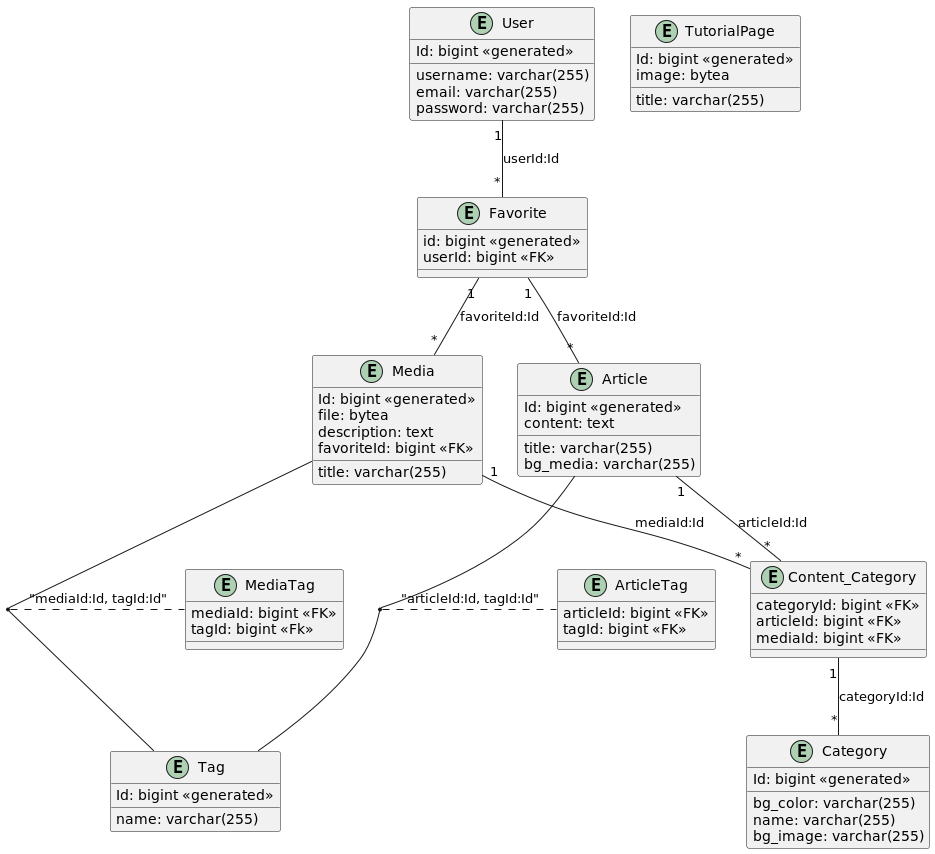
\includegraphics[height=1\textwidth]{./pics/erd.png}
    \caption{ERD}

  \end{figure}
\end{spacing}


\section{Medias und Articles}

Grundsätzlich haben wir als Team entschieden,
die Artikeln und die Medien in zwei speraten Tabellen zu speichern,
da Artikeln mehrere Bilder, Videos und Audios Inhalte enthalten können.
Diesen können dann mittels ein "Rich Text Editor" hinzugefügt werden.
Bei "Media" handlet es sich nur um ein Medienelement,
nähmlich ein Bild, Video oder Audio File. Es ist aber wichtig anzumerken,
dass keine Benutzeroberfläche für die Artikeln implementiert wurde, da der Kunde
diese nicht in dem \textbf{M}inimal \textbf{V}iable \textbf{P}roduct (MVP) haben wollte.
Für die Relaisierung des kompletten Datenmodels war aber das Einfügen der Artikel erforderlich.

\section{TutorialPage}
Die Entität "TutorialPage" hat keine Beziehungen zu anderen Entitäten, da sie nur für den Inhalt des Tutorial-Slideshows,
die nach der erfolgreichen Installation der App angezeigt wird, gedacht ist.

\begin{figure}[H]
  \centering
  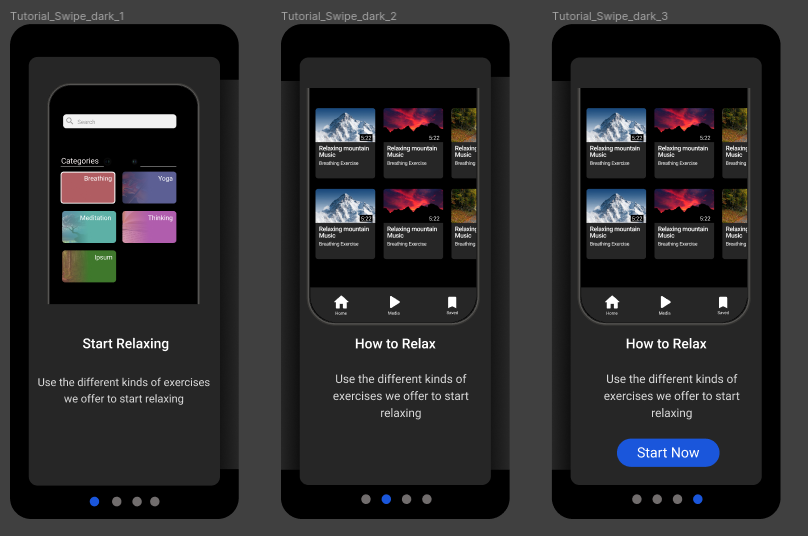
\includegraphics[height=0.5\textwidth]{./pics/slideshow.png}
  \caption{Screenshot aus dem UI Prototyp von Relaxoon}
\end{figure}

Mit der Persestierung der Inhalte von der Slideshow könnte die Erstellung
von neuen Builds bei jeder Änderung vermieden werden.


\section{Suche und Filterungen}

Bei den Filterungen wurde der "Interactive Query Builder" verwendet,
um die Filterparameter der Abfragen zu generieren
und diese dann bei den REST Abfragen anzuhängen.
Es gibt auch eine "Query Engine", welche die gleiche Funktion wie diese
"Interactive Query Builder" hat.
Diese kann in dem \textbf{O}bject \textbf{R}elational \textbf{M}apper (ORM) angewendet werden.
Mit der Verwendung dieser "Interactive Query Builder" kann man die Daten,
die man von den REST-Resourcen bekommt, anpassen.
Es gibt auch die Möglichkeit, die REST-Resource im Backend mittels dieser
"Query Engine" anzupassen.
Allerdings wurde diese "Query Engine" nicht verwendet,
da die Dokumentation bzw. Intellisense von dem ORM sehr ungenau war.

\begin{figure}[H]
  \centering
  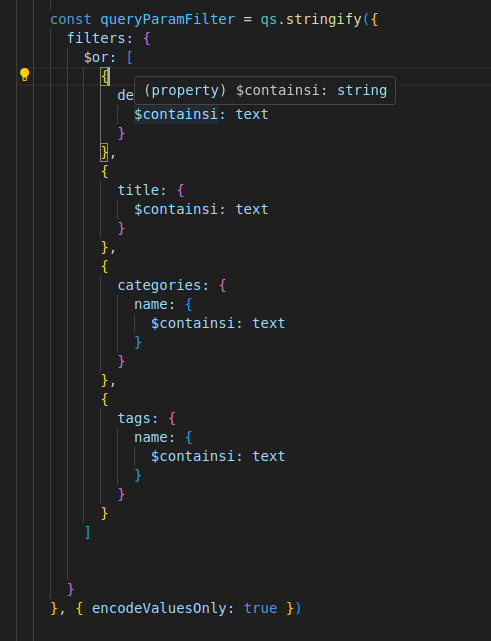
\includegraphics[ width=1\textwidth]{./pics/query-builder.png}
  \caption{Beispiel für den Interactive Query Builder}
\end{figure}




\begin{spacing}{1}
  \textbf{API-Route mit den angehängten generierten Abfrageparameter}:
  \newline
  \textcolor{red}{/medias?\&populate[tags]=true
  \&populate[file]=true
  \&populate[favorite][populate]=\newline users\_permissions\_user}
\end{spacing}


\section{State Management}
\begin{quotation}
  ``
  Der Begriff State ist in React-Applikationen überall präsent. Generell
  bezeichnet State den Zustand einer Komponente,
  also die dynamischen Daten, die eine Komponente den Benutzer:nnen anzeigt.
  Eine Änderung am State führt dazu, dass die Komponente neu gerendert wird
  und so die Datenänderung für die Benutzer:in sichtbar wird.
  Im einfachsten Fall verwaltet jede Komponente ihren eigenen State.
  Es gibt Fälle, in denen es jedoch erforderlich wird,
  den State zwischen mehreren Komponenten zu teilen.
  ''
  \cite{state-management}

  Um die Zustände der Applikation zu behandeln wurde meistens mit dem `useState Hook` von React gearbeitet.
  Der Einsatz einer State Management Library wie zum Beispiel RXJS oder Redux war gar nicht nötig, da die Anzahl der verwendeten UI-Komponenten nicht so groß ist.

  \subsection{useState Hook}
  ``useState is a React Hook that lets you add a state variable to your component.'' \cite{useState}


  \section{Dark/Light Mode}
  Da das Team sich für die Verwendung von der UI\-Library 'Native Base' entschieden hat, war die Realisierung von diesem Feature sehr einfach.
  Die Komponenten von 'Native Base' haben die Properties \_light und \_dark, wo man die Farbe einer Komponente je nach Modus definieren kann.
  Native Base verwendet im Hintergrund einen useContext Hook, wo die Modi der Applikation gespeichert werden.
  \subsection{useContext Hook}
  \begin{quotation}
    ``
    useContext is a React hook that provides a way to share data (context)
    across multiple components without explicitly passing it through props.
    It is part of the React Context API, which is built into the React library.
    '' \cite{useContext}

  \end{quotation}




\end{quotation}

\section{Help und Info Screen}

Mit der Speicherung der Inhalten von den Ansichten ''Help'' und ''Info''  ist neues Build für das Frontend nicht mehr nötig.
Somit kann der Content-Manager mehrere Freiheiten haben.
Diese Inhalte wurden mit sogenannten ''Single Types'' persestiert.
Ein ''Single Type'' ist nichts anders als eine Tabelle, die nur eine Zeile enthält.
Bei einer Änderung des Werts von diesem ''Single Type'' wird diese eine Zeile aktualisiert.

\section{Authentifizierung}
Für die Authentifizierung wurde mit Json Web Token (JWT) gearbeitet. Die Authentifizierungslogik im Server ist im Strapi eingebaut.Für den Client wurde die Logik so umgesetzt, dass der User die App erst verwenden kann, wenn er bereits authentifiziert ist.
Die Ansicht fürs Login soll aber nicht angezeigt werden, wenn der User bereits authentifiziert ist.
Umzu überprüfen, ob der Nutzer noch eingeloggt ist oder nicht wurde das Token im AsyncStorage gespeichert. Dieser ist ähnlich zu dem localStorage in der Webentwicklung. Somit wurde bei der Öffnung der App geprüft, ob das Token valid und nicht abgelaufen ist.
Damit der User auf die anderen Screens nicht zugreifen kann, wenn er nicht eingeloggt ist, wurde eine boolische Zustandsvariable verwendet, welche das LoginScreen als die zweite Ebene unserer Stack-Navigation rendert, wenn das Token invalid oder abgelaufen ist. Die erste Ebene ist für den TutorialScreen reseviert
Im folgenden Codestück ist die ganze Logik der Authentifizierung zu finden:
\begin{lstlisting}[caption=protected screens]
  import { createBottomTabNavigator } from '@react-navigation/bottom-tabs';
  import { createStackNavigator } from '@react-navigation/stack';
  import { useColorMode } from 'native-base';
  import * as React from 'react';
  import { useEffect, useState } from 'react';
  import { jwtDecode } from 'jwt-decode';
  import CategoryScreen from './screens/CategoryScreen';
  import HomeScreen from './screens/HomeScreen';
  import MediaScreen from './screens/MediaScreen';
  import SavedScreen from './screens/SavedScreen';
  import SettingsScreen from './screens/SettingsScreen';
  import VideoScreen from './screens/VideoScreen';
  import WaitScreen from './screens/WaitScreen';
  import HelpScreen from './screens/setting tabs/HelpScreen';
  import InfoScreen from './screens/setting tabs/InfoScreen';
  import { getToken } from './util/getUser';
  import TabBar from './components/TabBar';
  import TutorialScreen from './screens/intro/TutorialScreen';
  import LoginScreen from './screens/registration/LoginScreen';
  import RegistrationForm from './screens/registration/RegistrationForm';
  import { colors } from './styles/ThemeColors';
  import AsyncStorage from '@react-native-async-storage/async-storage';
  // Screen names
  type PageSettings = Record<string, { iconName: string; screen: React.ComponentType<any> }>;
  const settingsForScreenName: PageSettings = {
    Home: { iconName: 'home', screen: HomeScreen },
    Media: { iconName: 'play', screen: CategoryScreen },
    Saved: { iconName: 'list', screen: SavedScreen }
  };
  
  const Tab = createBottomTabNavigator();
  const Stack = createStackNavigator();
  
  function MainContainer(): JSX.Element {
    const { colorMode } = useColorMode();
    const [tokenExists, setTokenExists] = useState<boolean>(false);
    useEffect(() => {
      getToken()
        .then((data) => {
          console.info(typeof data);
          if (!data) throw new Error('no token');
          const decodedToken: { iat: number; exp: number; id: number } = jwtDecode(data);
          const eighthoursAfterNow = new Date(new Date().getHours() + 8).getMilliseconds();
          if (decodedToken.exp < eighthoursAfterNow) {
            setTokenExists(false);
            AsyncStorage.clear();
            return;
          }
          setTokenExists(true);
        })
        .catch((e) => {
          console.info('no token', e);
          setTokenExists(false);
        });
      console.info(tokenExists);
    }, []);
  
    return (
      <Stack.Navigator
        screenOptions={{
          headerShown: false
        }}
      >
        {/*
        <Stack.Screen name={"WaitScreen"} component={WaitScreen}/>
  */}
        {/*
        {!tokenExists && <Stack.Screen name="Tutorial" component={TutorialScreen}/>}
  */}
        {!tokenExists && <Stack.Screen name="Login" component={LoginScreen} />}
        {!tokenExists && <Stack.Screen name="Registration" component={RegistrationForm} />}
        <Stack.Screen
          name="Main"
          options={{
            headerShown: false
          }}
        >
          {() => (
            <Tab.Navigator
              screenOptions={{
                headerShown: false,
                headerTitleStyle: {
                  fontSize: 16,
                  color: colorMode === 'dark' ? colors.fontDark : colors.fontLight
                }
              }}
              tabBar={(props) => <TabBar color={colorMode} {...props} />}
            >
              {Object.entries(settingsForScreenName).map(([pageName, settings]) => (
                <Tab.Screen key={pageName} name={pageName} component={settings.screen} />
              ))}
            </Tab.Navigator>
          )}
        </Stack.Screen>
        <Stack.Screen name="Content" component={MediaScreen} />
        <Stack.Screen component={VideoScreen} name="Video" />
        <Stack.Screen component={SettingsScreen} name="Settings" />
        <Stack.Screen name="Info" component={InfoScreen} />
        <Stack.Screen name="Help" component={HelpScreen} />
      </Stack.Navigator>
    );
  }
  
  export default MainContainer;
    
\end{lstlisting}

\section{Validierung}
Strapi an sich hat eine eingebaute Validierung für Emails und Passwörter. Das Team hat aber eine client-seitige Validierung implementiert, um die Anzahl der Requests zu minimieren und eine bessere UX zu schaffen.
Für die client-seitige Validierung wurde eine Library namens 'Zod' verwendet. Diese verwendet Builder Pattern um ein Validierungsschema zu bauen.
\begin{lstlisting}[caption=Validierungsschemen]
 import { z } from 'zod';

export const nameValidator = z.string().min(3);
export const emailValidator = z.string().email();
export const passwordValidator = z.string().min(6);
  
\end{lstlisting}


\section{Deployment}

\subsection{Allgemeins}

Die Veröffentlichung der Applikation auf den Play Stores wurde von dem Auftraggeber nicht in die Frage gestellt.
Das Hochladen der Android-Applikation auf Firebase App Distribution wurde aber von dem Team verlangt.
Das Backend wurde auf den Servers der Firmen Solvistas und Macolution deployt. Für Demonstrationszwecke wurde ein lokales Deployment auf Minikube erstellt
% Die Firmen Solivstas und Macolution wollten das Endpordukt auf ihrer eigenen
% Infrastruktur deployen und die Anwendungen
% als Docker-Images in den Container-Registries von denen speichern.
% Da die genannten Firmen keine Zugriffsrechte für das Team organisiert haben,
% war es für das Team schwierig, beim finalen Deployment mitzumachen. Das Team hat aber die Möglichkeit gehabt,
% beim Deployment auf dem Stagingsystem mitzuhelfen, da die Software auf einem externen Service, nämlich
% Firebase App Distribution, hochgeladen wurde.
% Der Betreuer wurde ebensfalls informiert und er verlangte ein lokales Deployment für das Backend mittels ''Minikube'' sowie ein Live-Demo für die Applikation auf einem Emulator


% \subsubsection{Container Registry}

% \begin{quotation}
%   ``
%   A container registry is a repository—or collection of repositories—used to store and access container
%   images. Container registries can support container-based application development,
%   often as part of DevOps processes.
%   Container registries can connect directly to container orchestration platforms like Docker and Kubernetes.
%   ''
%   \cite{container-registry}
% \end{quotation}




\subsection{Deployment Diagram}
\begin{center}
  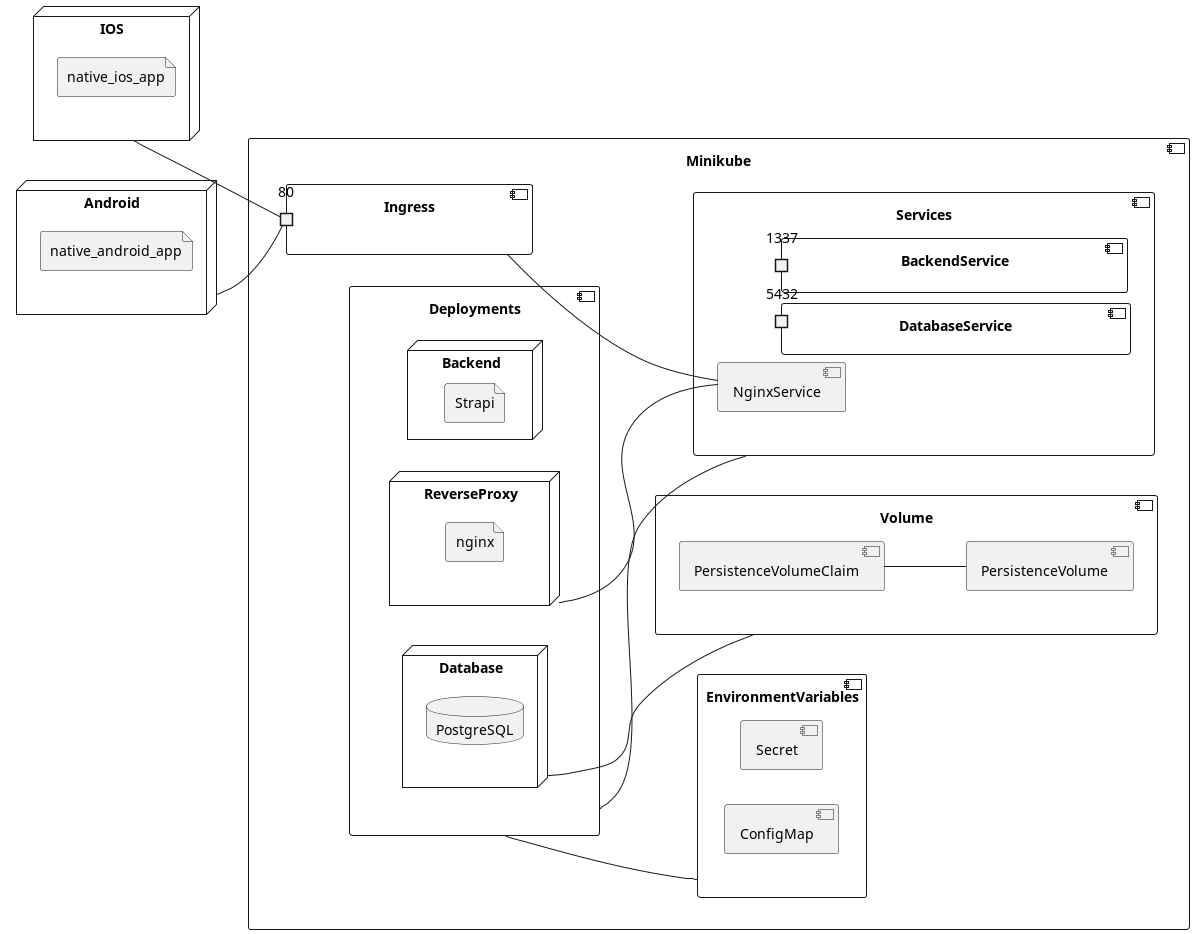
\includegraphics[width=\textwidth]{pics/dev-deployment.png}
\end{center}
\subsection{Deployment von dem Backend auf Minikube}

Damit ein funktionsfähiges Deployment erstellt werden kann sind solche Komponenten zu deployen:
\begin{itemize}
  \item Strapi
  \item Datenbank
  \item Reverse Proxy (Nginx)
\end{itemize}

Für jede dieser genannten Bauteile des Backends sind K8S- (Kubernetes) Deployments und Services zu erstellen.

\subsection{K8S-Konfigurationen für die Datenbank}
Zusätzlich zu einer Deployment- und Service-Kompoente ist für die Sicherung
von den Credentials der Datenbank eine sogenannte
Secret-Komponente gebraucht.
Für die Vermeidung von Datenverlusten in Fällen
wie Neustart eines Pods oder die Aktualisierung
der Konfiguration von dem Pod ist
das Anglegen einer PersistenceVolume-Komponente sehr dringend
Damit das Deployment auf die PersistenceVolume-Komponente zugreifen kann, ist eine sogenannte PersistenceVolumeClaim-Komponente zu definieren

Für die Konfiguration der Secret-, Service- und Deployment-Komponente wurde die kubectl \textbf{C}ommand \textbf{L}ine \textbf{I}nterface verwendet.
Die PersistenceVolume-Komponente bzw. die PersistenceVolumeClaim-Kompoente wurden fertige Konfigurationen genommen
\begin{lstlisting}[caption=K8S PVC]
  apiVersion: v1
  kind: PersistentVolumeClaim
  metadata:
    finalizers:
    - kubernetes.io/pvc-protection
    name: strapi-pvc
    namespace: default
  spec:
      accessModes:
        - ReadWriteMany
      resources:
        requests:
          storage: 10Mi
      storageClassName: standard
    
\end{lstlisting}


\begin{lstlisting}[caption=K8S PV]
  apiVersion: v1
  kind: PersistentVolume
  metadata:
    finalizers:
    - kubernetes.io/pv-protection
    labels:
      type: local
    name: strapi-volume
    resourceVersion: "33077"
    uid: ae6d772a-0090-4074-b3ac-1edb929daf29
  spec:
    accessModes:
    - ReadWriteOnce
    capacity:
      storage: 10Gi
    hostPath:
      path: /mnt/data
      type: ""
    persistentVolumeReclaimPolicy: Retain
    storageClassName: manual
    volumeMode: Filesystem
  status:
    phase: Available
    
\end{lstlisting}



\subsection{K8S-Konfigurationen für Strapi}
Für Strapi wird auch eine Secret-Komponente benötigt, da der Server geheime Umgebungsvariablen benötigt.
Es gibt auch einige.
Damit das Deployment von Strapi erstellt werden kann, muss die Anwendung zuerst containerisiert werden. Dies kann erfolgen mit der Verwendung des folgenden Dockerfiles .
\begin{lstlisting}[caption=Strapi Dockerfile]
  # Creating multi-stage build for production
  FROM node:18-alpine as build
  RUN apk update && apk add --no-cache build-base gcc autoconf automake zlib-dev libpng-dev vips-dev git > /dev/null 2>&1
  ARG NODE_ENV=production
  ENV NODE_ENV=${NODE_ENV}
  
  WORKDIR /opt/
  COPY package.json package-lock.json ./
  RUN npm install -g node-gyp
  RUN npm config set fetch-retry-maxtimeout 600000 -g && npm install --only=production
  ENV PATH /opt/node_modules/.bin:$PATH
  WORKDIR /opt/app
  COPY . .
  RUN npm run build
  # Creating final production image
  FROM node:18-alpine
  RUN apk add --no-cache vips-dev
  ARG NODE_ENV=production
  ENV NODE_ENV=${NODE_ENV}
  ENV HOST=0.0.0.0
  ENV PORT=1337
  ENV APP_KEYS=secret
  ENV API_TOKEN_SALT=secret
  ENV ADMIN_JWT_SECRET=secret
  ENV TRANSFER_TOKEN_SALT=secret
  # Database
  
  # Database
  ENV DATABASE_CLIENT=postgres
  ENV DATABASE_HOST=localhost
  ENV DATABASE_PORT=5432
  ENV DATABASE_NAME=strapi
  ENV DATABASE_USERNAME=strapi
  ENV DATABASE_PASSWORD=strapi
  ENV DATABASE_SSL=false
  ENV JWT_SECRET=cVRog3q5woTNB8EJ+vKPFA==
  
  
  
  
  WORKDIR /opt/
  COPY --from=build /opt/node_modules ./node_modules
  WORKDIR /opt/app
  COPY --from=build /opt/app ./
  ENV PATH /opt/node_modules/.bin:$PATH
  
  RUN chown -R node:node /opt/app
  USER node
  EXPOSE 1337
  CMD ["npm", "run", "start"]
    
\end{lstlisting}

Dieses Image soll dann in einem Container Registry wie zum Beispiel
Dockerhub oder Github Container Registry hochgeladen werden,
damit die K8S-Deployment-Komponente dieses Image im Einsatz nimmt.




\subsection{K8S-Secrets}
Damit man Umgebungsvariablen in einem K8S-Cluster definieren kann gibt es zwei Möglichkeiten.
Man kann entweder eine ConfigMap-Komponente verwenden oder eine Secret-Komponente. Es gibt auch die Möglichkeit, diese Umgebungsvariablen direkt in den Konfigurationen von der Deployment-Komponente händisch einzutragen.
Für geheime bzw. sensible Daten werden K8S-Secrets verwendet.
Das Anlegen der benötigten Secrets für unsere Anwendung erfolgte durch die Verwendung folgender Befehle
\begin{lstlisting}[caption=Secrets für Strapi]
    kubectl create secret generic strapi-server-secret \
  --from-literal=PORT=1337 \  
  --from-literal=APP_KEYS=secret
  --from-literal=API_TOKEN_SALT=secret \
  --from-literal=ADMIN_JWT_SECRET=secret \
  --from-literal=TRANSFER_TOKEN_SALT=secret \
  --from-literal=DATABASE_CLIENT=postgres \
  --from-literal=DATABASE_PORT=5432 \
  --from-literal=DATABASE_NAME=secret \
  --from-literal=DATABASE_USERNAME=secret \
  --from-literal=DATABASE_PASSWORD=secret \
  --from-literal=DATABASE_SSL=false \
  --from-literal=JWT_SECRET=secret
\end{lstlisting}


\begin{lstlisting}[caption=Secrets für die Datenbank]
kubectl create secret generic  strapi-secret \
--from-literal=POSTGRES_USER=strapi \
--from-literal=POSTGRES_PASSWORD=strapi \
--from-literal=POSTGRES_DB=strapi
\end{lstlisting}








\subsection{Was ist eine Deployment-Komponente}

Eine Deployment-Komponente dient dazu, dass ein Pod erstellt wird und die benötigten Resourcen bzw. Volumes und Zugriffsrechten
dafür definiert werden.\cite{k8s-deployment}

Für das Anlegen einer Deployment-Komponente muss man zuerst die Anwendung containerisieren.
Für weit verbreitete Software wie z.B.: PostgreSQL gibt es bereites viele vorhandene Images auf unterschiedliche Container-Registries

Folgende Befehle wurden verwendet, um die Deployment-Komponenten für Strapi und PostgreSQL zu erstellen:

\begin{lstlisting}[language=bash, caption=create k8s deployments]
kubectl create deployment relaxoon-db --image=postgres:12.16-bullseye --port=5432
kubectl create deployment relaxoon-strapi --image=ghcr.io/Abdulrahman-AL-Sabagh/relaxoon-strapi:latest --port=8080
    
\end{lstlisting}


\subsubsection{Was ist ein Pod}

\begin{quotation}
  ``
  Ein Pod (übersetzt Gruppe/Schote, wie z. B. eine Gruppe von Walen oder eine Erbsenschote)
  ist eine Gruppe von einem oder mehreren Containern mit gemeinsam genutzten Speicher- und
  Netzwerkressourcen und einer Spezifikation für die Ausführung der Container.
  Die Ressourcen eines Pods befinden sich immer auf dem gleichen (virtuellen) Server,
  werden gemeinsam geplant und in einem gemeinsamen Kontext ausgeführt.
  Ein Pod modelliert einen anwendungsspezifischen "logischen Server": Er enthält eine oder mehrere
  containerisierte Anwendungen, die relativ stark voneinander abhängen.
  ''
  \cite{pod}
\end{quotation}






\subsection{Erstellung einer Service-Komponente}

Mit dem Einsatz eines Services in Kubernetes können Pods,
die sich im gleichen Cluster befinden,miteinander kommunizieren. \cite{k8s-service}

Für das Anlegen einer Service-Komponente kann man diesen Befehl nutzen:

\begin{lstlisting}[language=bash,caption=create a service component]
kubectl expose deployments/<Name des Pods> --port=5432
\end{lstlisting}






\subsection{Erstellung einer Ingress-Komponente}

Damit der Emulator, der sich außerhalb des lokalen Clusters von Minikube befindet,
mit dem deployten Backend kommunizieren kann,
ist das Anlegen einer Ingress notwendig.

//TODO Config für die Ingress-Komponente noch hingeben

//TODO Dieses Kapitel noch fertigschreiben



``
In einem Computernetzwerk befindet sich ein einfacher Reverse-Proxy zwischen einer
Gruppe von Servern und den Clients, die sie verwenden wollen.
Als Client gilt jede Hardware oder Software, die Anfragen an einen Server senden kann. [...].
Der Reverse-Proxy fängt alle Anfragen von den Clients an die Server ab und liefert auch
alle Antworten und Dienste von
en Servern wieder an die Clients zurück. Aus Sicht des Kunden sieht es so aus,
als würde alles von einer einzigen Stelle ausgehen.

''
\cite{reverse-proxy}

\subsection{Buildprozess für das Frontend}

Damit man das Frontend deployt, muss man zuerst den nativen Android und IOS Code generieren.
Danach sollen die Android bzw. IOS Anwendungen mit einer IDE oder mit der Kommando-Zeile gebaut werden.
Um den nativen Code zu generieren ist folgendes einzugeben:
\begin{lstlisting}[language=Bash,caption=generate android and ios]
npx expo prebuild
\end{lstlisting}





\subsection{Erstellung einer .apk Datei}
Für Android wurde die .\textbf{A}ndroid \textbf{P}ac\textbf{K}age (apk)  mit dem Einsatz von gradle Wrapper generiert.
Foglendes muss installiert und richtig konfiguriert werden, damit  eine .apk Datei generierbar ist:



\begin{itemize}
  \item Java 11
  \item Installation von sdkmanager
  \item Lizenzen von sdkmanager müssen akzeptiert sein
  \item Installation von einer Android SDK
  \item Konfigurationen für JAVA\_HOME und ANDROID\_HOME
  \item Installation einer CLI namens "ninja"
\end{itemize}

Der Generierungsbefehl für die Build-Datei schaut dann wie folgendes aus:

\begin{lstlisting}[language=bash,caption=generate apk]
 ./gradlew assembleRelease
 \end{lstlisting}





\section{Hochladen einer Mobileapp auf Firebase App Distribution}

Nachdem Anlegen eines Accuonts bei Firebase sind folgende und die Erstellung eines Projektes Schritte zu machen:


\begin{figure}
  Damit die benötigten Firebase Services für die Applikationen aktiviert werden, muss man zuerst die benötigten Konfigurationen eingeben.
  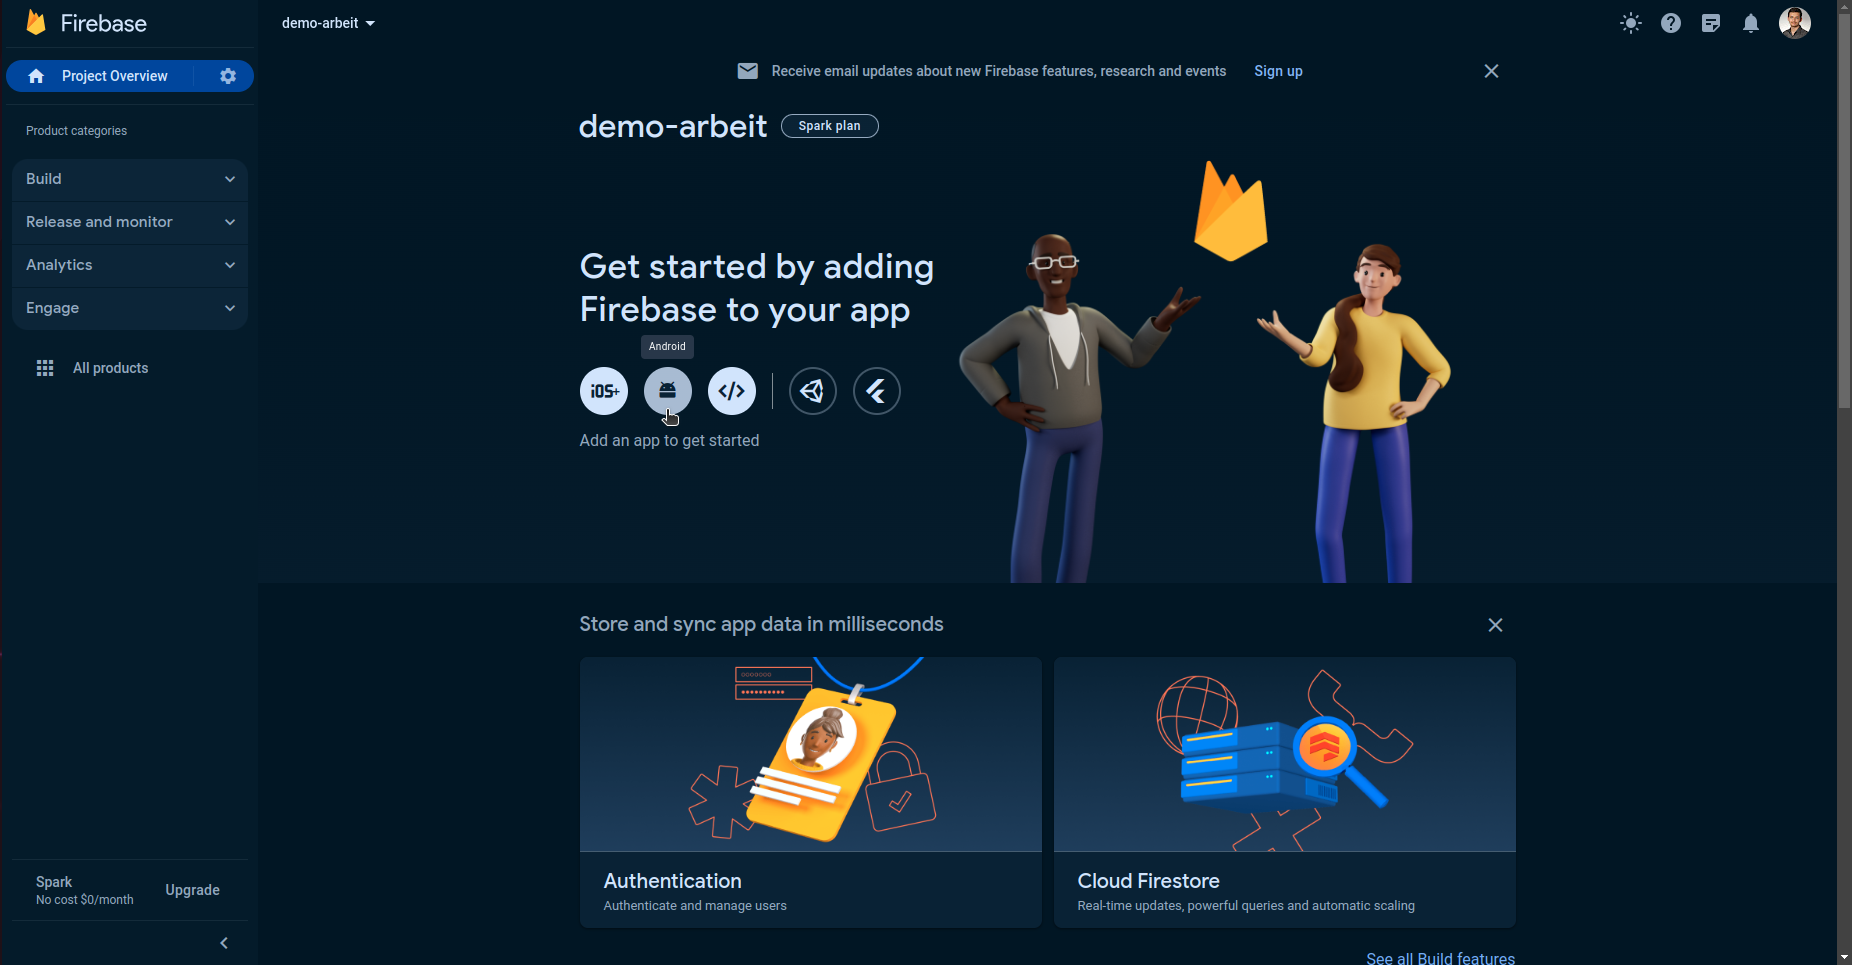
\includegraphics[width=\textwidth]{./pics/firebase1.png}
  \caption{create android config}
\end{figure}



\begin{figure}
  Folgende Daten müssen eingegeben werden, damit die Firebase Services für die Android Applikation eingeschaltet werden können.

  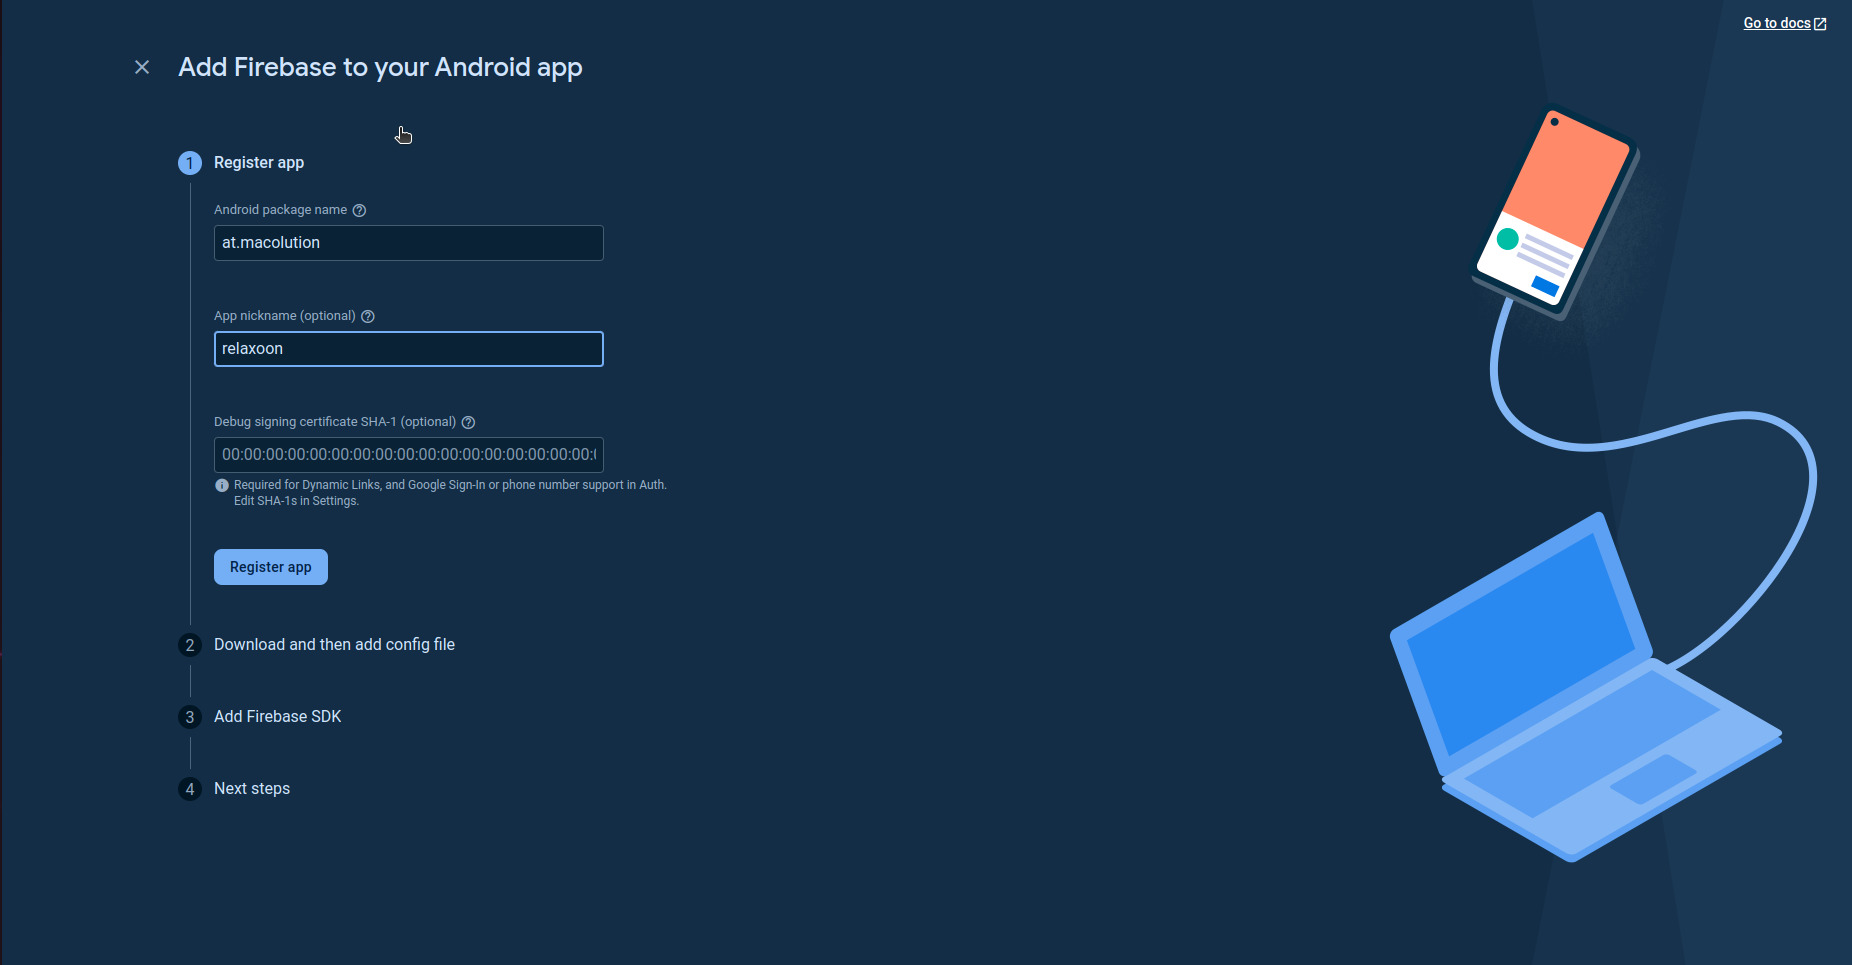
\includegraphics[width=\textwidth]{./pics/firebase2.png}
  \caption{Android Config}
  Die restlichen Punkte sind für das Projekt Relaxoon irrelevant,
  da die Firebase-SDK in der vorleigende Arbeit nicht eingesetzt wird.
\end{figure}



\begin{figure}
  Danach soll man  auf die App Distribution gehen und dann auf ''Get Started'' klicken
  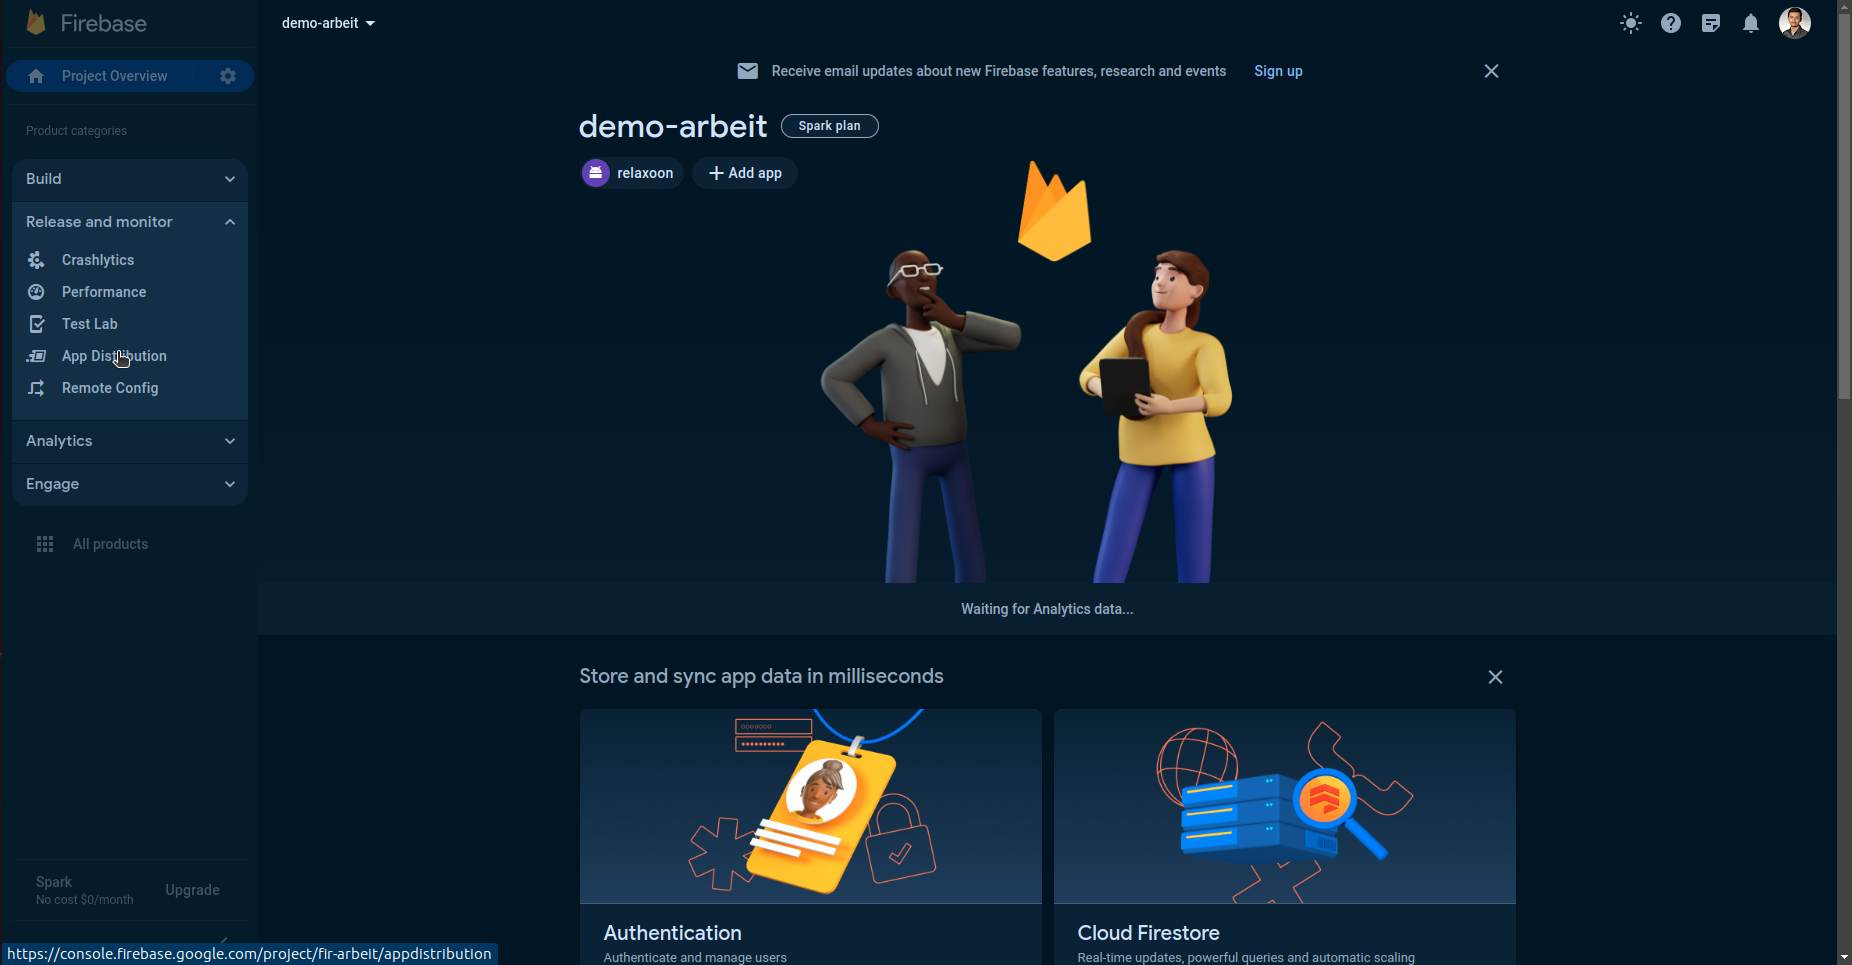
\includegraphics[width=\textwidth]{./pics/firebase3.png}
  \caption{App Distribution}
\end{figure}

\begin{figure}
  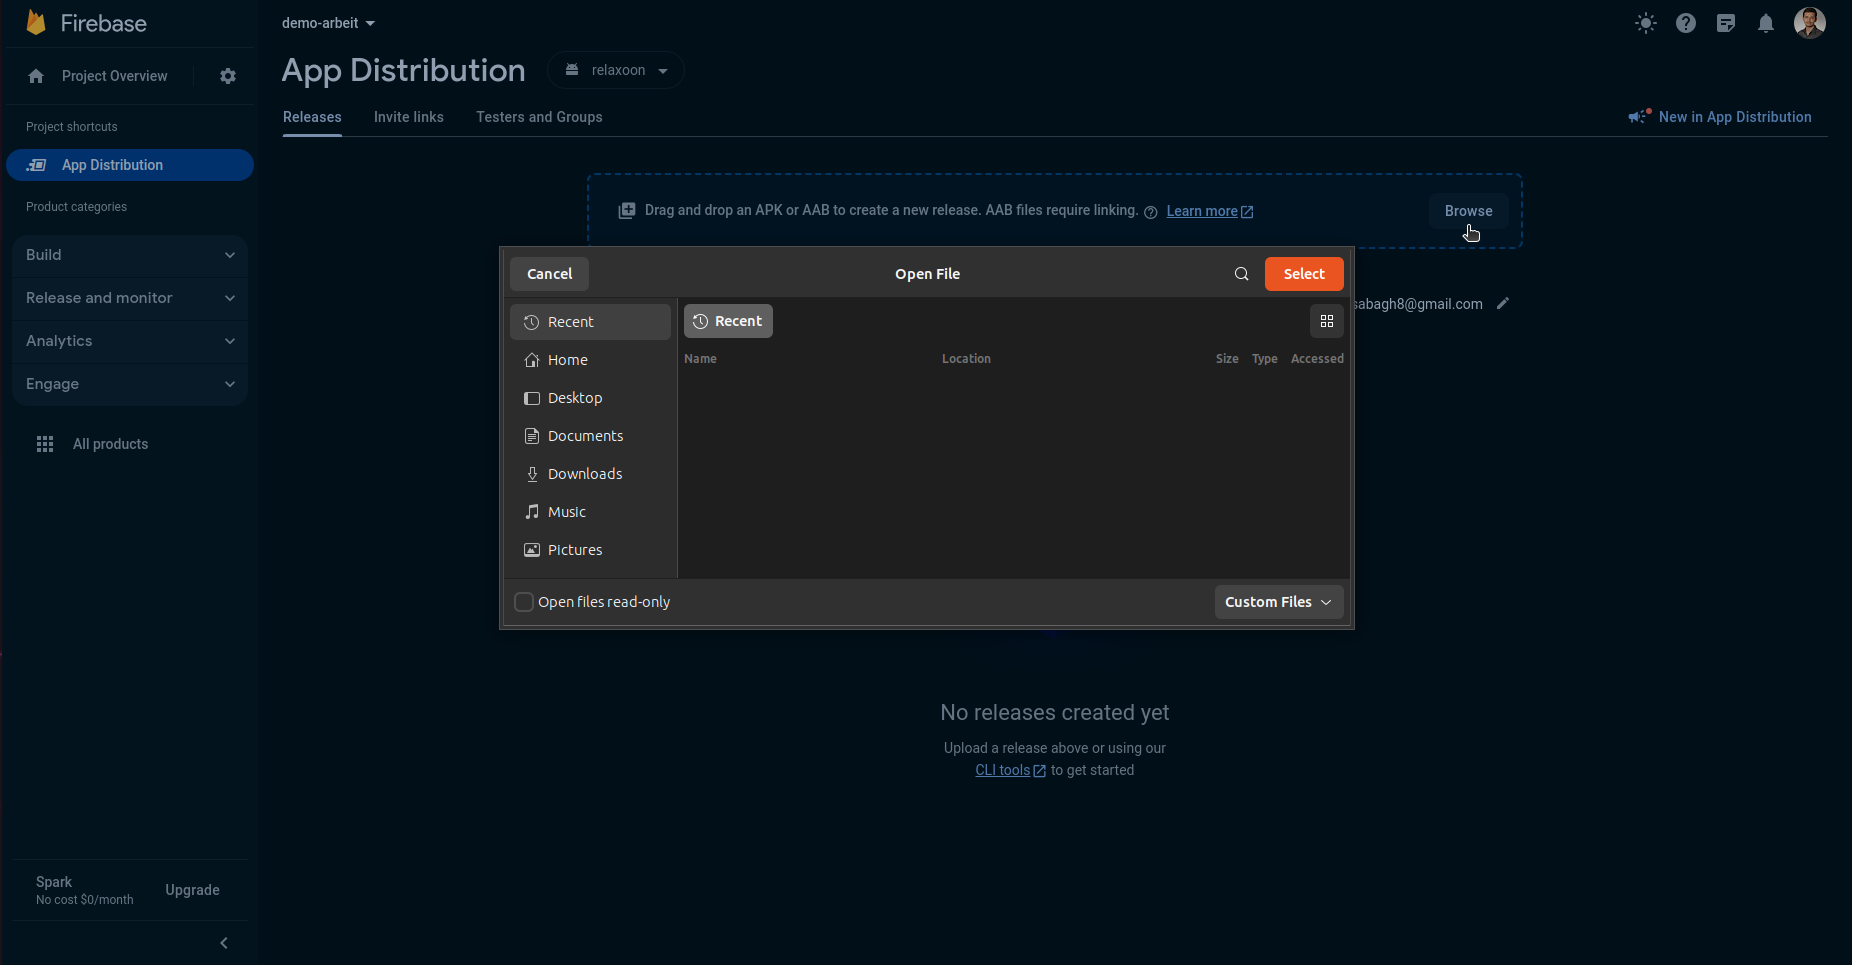
\includegraphics[width=\textwidth]{./pics/firebase4.png}
  \caption{App upload}
  Die App kann mit diesem ''Browse Fenster'' oder mit ''Drag and Drop'' hochgeladen werden

\end{figure}



\begin{figure}
  Das Produkt kann dann an anderen TestUsers verteilt werden, indem man die Email-Adressen dieser Testers beim Release eingibt.
  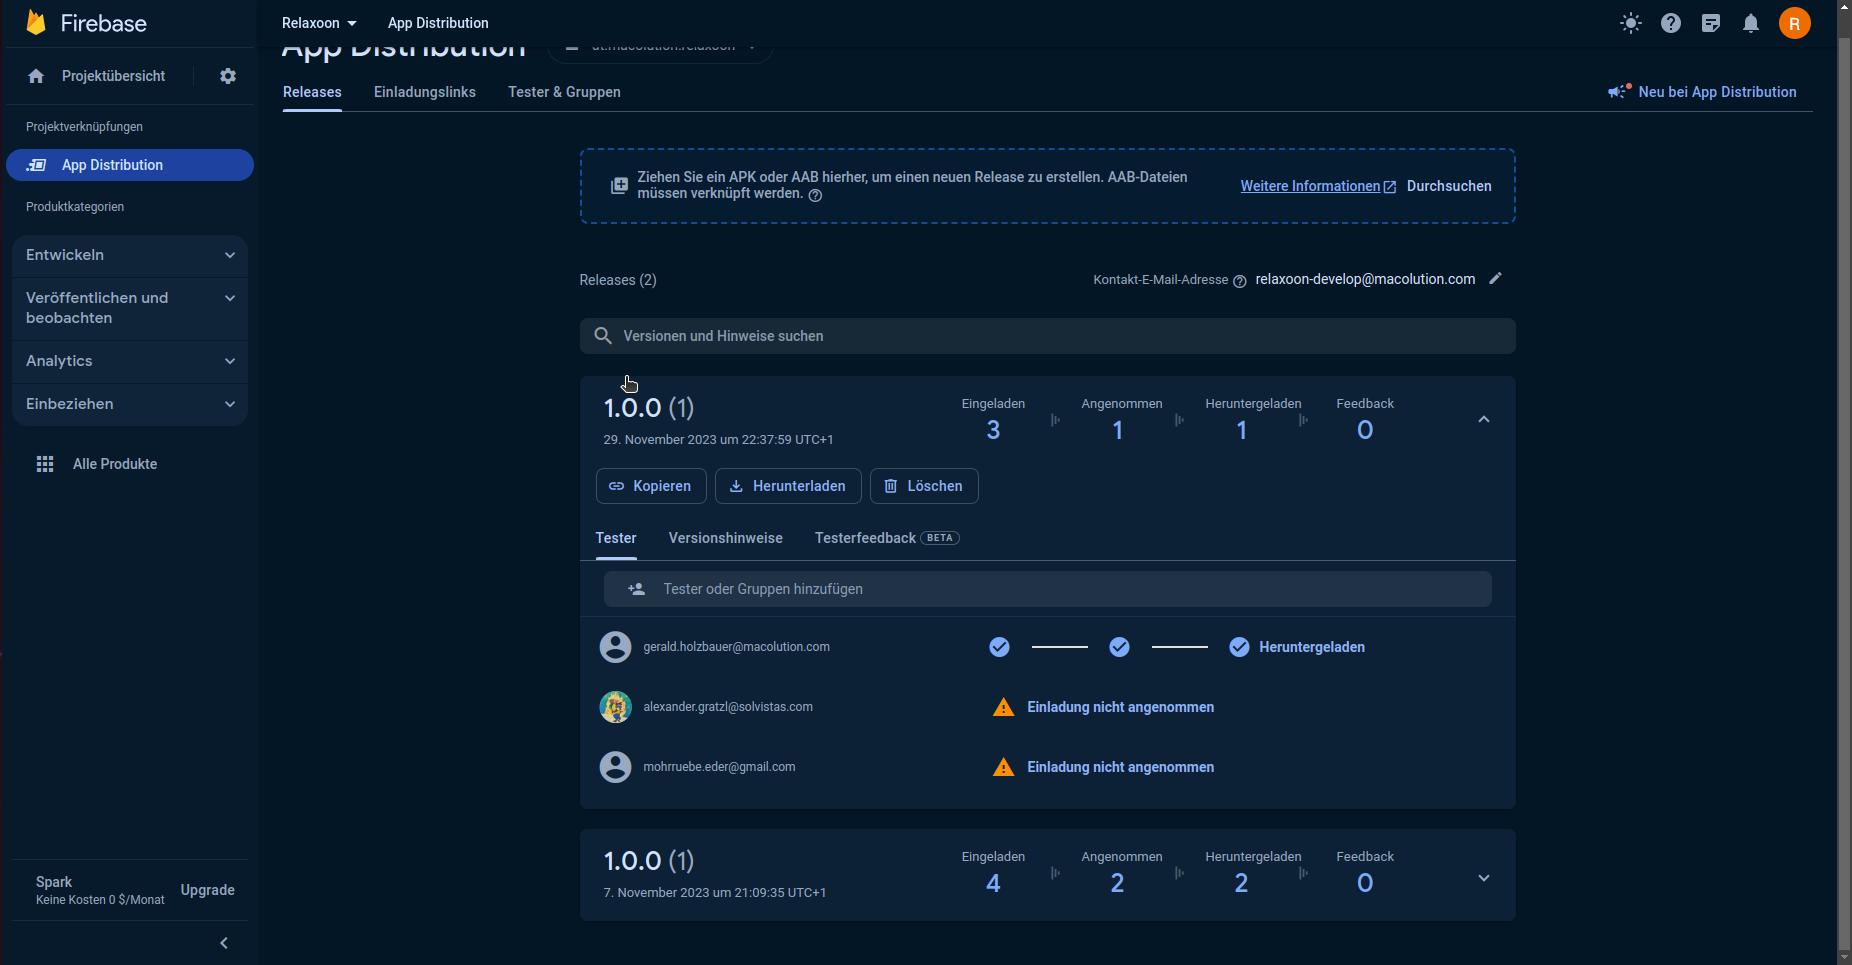
\includegraphics[width=\textwidth]{./pics/firebase5.png}
  \caption{releases}
\end{figure}

